\definecolor{tclblue}{HTML}{2A78D6}
\definecolor{tclorange}{HTML}{EB6834}
\definecolor{tclgray}{HTML}{8A8984}

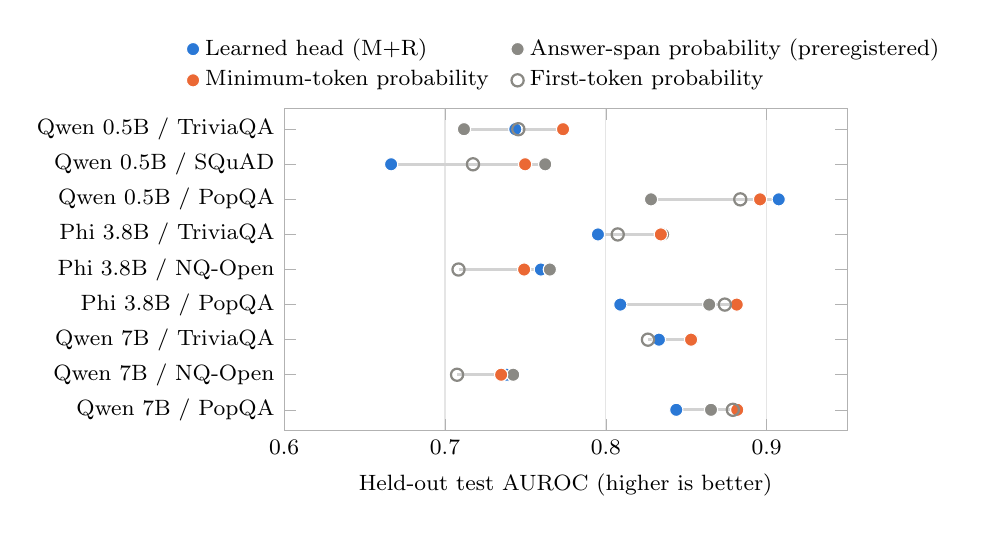
\begin{tikzpicture}
\begin{axis}[width=0.72\textwidth, height=5.68cm, xmin=0.6, xmax=0.95, ymin=0.4, ymax=9.6, ytick={1,...,9}, yticklabels={{Qwen 0.5B / TriviaQA},{Qwen 0.5B / SQuAD},{Qwen 0.5B / PopQA},{Phi 3.8B / TriviaQA},{Phi 3.8B / NQ-Open},{Phi 3.8B / PopQA},{Qwen 7B / TriviaQA},{Qwen 7B / NQ-Open},{Qwen 7B / PopQA}}, y dir=reverse, xtick={0.6,0.7,0.8,0.9}, xmajorgrids, major grid style={gray!20}, tick label style={font=\footnotesize}, label style={font=\footnotesize}, axis line style={gray!60}, tick style={gray!60}, xlabel={Held-out test AUROC (higher is better)}, legend style={font=\footnotesize, at={(0.5,1.02)}, anchor=south, legend columns=2, legend cell align=left, draw=none, /tikz/every even column/.append style={column sep=6pt}}]
\draw[gray!35, line width=1.2pt] (axis cs:0.7118,1) -- (axis cs:0.7734,1);
\draw[gray!35, line width=1.2pt] (axis cs:0.6665,2) -- (axis cs:0.7623,2);
\draw[gray!35, line width=1.2pt] (axis cs:0.8281,3) -- (axis cs:0.9075,3);
\draw[gray!35, line width=1.2pt] (axis cs:0.7951,4) -- (axis cs:0.8357,4);
\draw[gray!35, line width=1.2pt] (axis cs:0.7084,5) -- (axis cs:0.7652,5);
\draw[gray!35, line width=1.2pt] (axis cs:0.8090,6) -- (axis cs:0.8814,6);
\draw[gray!35, line width=1.2pt] (axis cs:0.8262,7) -- (axis cs:0.8537,7);
\draw[gray!35, line width=1.2pt] (axis cs:0.7075,8) -- (axis cs:0.7424,8);
\draw[gray!35, line width=1.2pt] (axis cs:0.8438,9) -- (axis cs:0.8817,9);
\addplot[only marks, mark=*, mark size=2.4pt, fill=tclblue, draw=white] coordinates {(0.7437,1) (0.6665,2) (0.9075,3) (0.7951,4) (0.7596,5) (0.8090,6) (0.8330,7) (0.7385,8) (0.8438,9)};
\addlegendentry{Learned head (M+R)}
\addplot[only marks, mark=*, mark size=2.4pt, fill=tclgray, draw=white] coordinates {(0.7118,1) (0.7623,2) (0.8281,3) (0.8357,4) (0.7652,5) (0.8643,6) (0.8537,7) (0.7424,8) (0.8654,9)};
\addlegendentry{Answer-span probability (preregistered)}
\addplot[only marks, mark=*, mark size=2.4pt, fill=tclorange, draw=white] coordinates {(0.7734,1) (0.7498,2) (0.8959,3) (0.8342,4) (0.7492,5) (0.8814,6) (0.8530,7) (0.7349,8) (0.8817,9)};
\addlegendentry{Minimum-token probability}
\addplot[only marks, mark=o, mark size=2.2pt, draw=tclgray, thick] coordinates {(0.7456,1) (0.7174,2) (0.8836,3) (0.8074,4) (0.7084,5) (0.8740,6) (0.8262,7) (0.7075,8) (0.8790,9)};
\addlegendentry{First-token probability}
\end{axis}
\end{tikzpicture}
